\chapter{Building a Decentralized File Sharing Application}\label{chapter:building-dapp}

	\section{Introduction}
	Chapter~\ref{chapter::app-concepts-design} focused on different application concepts and showed the underlying architecture for building decentralized applications where users are in control of their data. This chapter focuses on analyzing the \textit{state-of-the-art} by building two \textit{proof-of-concept} applications for secure file sharing.
	
	\section{Problem Context}
	Existing applications for sharing files are central solutions and therefore suffer from single point of failure risk. Moreover, using central services for securing data means that we have to trust a 3rd party with our data thus exposing it to manipulation risks. Hence, a decentralized application is required to overcome the problems posed by a central application. With the recent developments in Blockchain technology and p2p storage, it is possible to securely store and share data without using any central server.
	
	\section{Requirements}
	A decentralized file sharing application should have following desirable properties:
	\begin{itemize}
		\item Client-side encryption.
		\item Encryption keys are in user's possession.
		\item Users can choose the data storage location.
		\item Easy and secure sharing of files with other users of the application.
	\end{itemize}

	\section{A File Sharing Application using Ethereum}
	This section describes the workings of the application \textit{dShare-ethereum}\cite{harsh_kedia_2019_3359852} built using p2p technologies enabling a secure way of storing and sharing data between two individuals or entities. The latest version of the application is deployed at \url{https://file-share-dapp.herokuapp.com/}
	
		\subsection{Use Case}
		Today’s supply chain spans multiple geographies, but the documents involved in the industry such as delivery certificates are still in physical form. This paperwork prevents manipulations but leads to various delays across the whole chain, thus affecting everyone involved\footnote{\url{https://www-01.ibm.com/common/ssi/cgi-bin/ssialias?htmlfid=XI912347USEN}}.
		
		The above problem can be solved by digitizing all documents, time-stamping them using a trusted Time stamping authority (TSA) and upload them to a cloud service. However, the tools used to accomplish this solution are central services, and, therefore, suffers from data manipulations by a 3rd party.
		
		We, therefore, need a solution that is peer-to-peer (P2P) and decentralized. Recent distributed technologies offers a means of decentralized time stamping and enables peer-to-peer storage systems that are resistant to manipulations by any 3rd party.
		
		\textit{dShare-ethereum} is built using decentralized technologies such as Bitcoin\cite{nakamoto2008bitcoin}, Ethereum\cite{buterin2014ethereum} and IPFS\cite{benet2014ipfs} such that it's capable of immutable timestamping and secure file sharing in a p2p fashion.
		
		\subsection{Technologies Used}
			\subsubsection{Ethereum}
			Ethereum\cite{buterin2014ethereum} is a blockchain platform for building decentralized applications. It allows the creation of \textit{Smart Contracts} which serves as a backend for the application. Solidity\footnote{\url{https://github.com/ethereum/solidity}} is the primary language for writing smart contracts on Ethereum.
			
			\subsubsection{InterPlanetary File System (IPFS)}
			IPFS is used as a decentralized storage for storing of files and their corresponding decryption key which are encrypted using the uploader's public key.
			
			\subsubsection{OriginStamp}
			OriginStamp\cite{hepp2018originstamp} is a blockchain based system for decentralized timestamping. It uses the Bitcoin blockchain for the creation of trusted and immutable timestamps for any piece of data. Timestamps created by OriginStamp can be verified independently by anyone.
			
			\begin{figure}[h]
				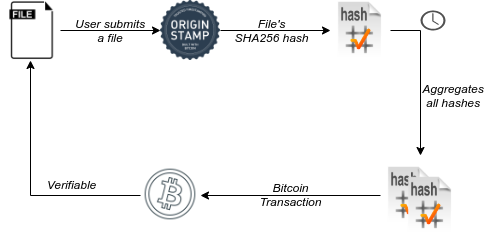
\includegraphics[width=\linewidth]{figures/origin-stamp}
				\caption{\label{fig:originstamp} Timestamping using OriginStamp}
			\end{figure}
			
			Figure~\ref{fig:originstamp} visualizes the timestamping process as implemented in OriginStamp. When a user submits a file, the hash of the data is recorded. It combines all the hashes submitted over a period of time and generates an aggregated hash. After some additional hashing and encoding operations, a Bitcoin address is created to which the smallest possible transactional amount of Bitcoins is transferred. Performing this transaction embeds the hash and the timestamp permanently to the Bitcoin blockchain. Each transaction is part of a block and is added to the Bitcoin blockchain by a process called mining. Since each block is linked cryptographically to the previous block, adding a new block confirms the validity of the last block. Changing the timestamp of a transaction becomes impossible once five or six subsequent blocks are mined, which requires an hour on average\cite{nakamoto2008bitcoin}.
			
			\subsubsection{Firebase}
			Firebase\footnote{\url{https://firebase.google.com/}} is used as a database for storing of user's public keys which is used for encryption of a file's key when it's shared with another user.
			
			\subsubsection{MetaMask}
			MetaMask\footnote{\url{https://metamask.io/}} is an Ethereum wallet. It serves as a web3\footnote{\url{https://web3js.readthedocs.io/}} provider allowing any application to interact with the Ethereum blockchain.
			
		\subsection{Application Architecture}
		
			\begin{figure}[h]
				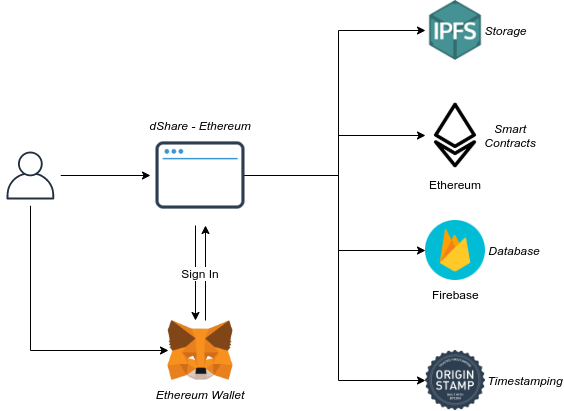
\includegraphics[width=\linewidth]{figures/dshare-ethereum}
				\caption{\label{fig:dshare-ethereum} \textit{dShare-ethereum} Architecture}
			\end{figure}
			
			Figure~\ref{fig:dshare-ethereum} visualizes the application architecture. User authentication is handled by MetaMask. For storing of files we used IPFS. Before uploading to the IPFS network, files are encrypted using AES-GCM\footnote{\url{https://www.aes-gcm.com/}} encryption mechanism. Sharing of encryption keys is facilitated using smart contracts built on Ethereum; thus files can be shared by anyone with an Ethereum address. Finally, OriginStamp is used for immutable timestamping.
			
			The front-end of the application is built using React.js\footnote{\url{https://reactjs.org/}}, a JavaScript library for building user interfaces. Solidity was used for writing smart contracts and deployed on the Ethereum test network, Rinkeby\footnote{\url{https://www.rinkeby.io}}. Next.js\footnote{\url{https://nextjs.org/}} was used for server-side rendering (SSR)\footnote{\url{https://nextjs.org/features/server-side-rendering/}}, and Firebase\footnote{\url{https://firebase.google.com/}} was used as a database for storing public Ethereum key of the users.
			
		\subsection{Working}
			\subsubsection{Authentication}
				When a user logs into the application, she is presented with a MetaMask dialog which asks her to sign a randomly generated value. This signature is used to retrieve the public key for the selected Ethereum address. The public key is then saved to the database and user is logged in.
			
			\subsubsection{Smart Contract}
				The smart contract serves as the bridge between the front-end of the application and the Ethereum Blockchain. Data is read from and written to the blockchain with the help of function calls in the contract. Each function call which modifies some data requires a small fee in the form of gas\footnote{\url{https://ethereum.stackexchange.com/questions/3/what-is-meant-by-the-term-gas}} which defines the cost for a function execution in Ether. Reading from the blockchain does not require any fees.
				
				The application makes use of two contracts, \textit{FileFactory}, which acts as the factory contract for creation of new files and \textit{File}, which represents an individual file. Code for both the contracts is available at \url{https://github.com/hKedia/dShare/blob/master/ethereum/contracts/FileShare.sol}
				
				\paragraph{FileFactory}
				\textit{FileFactory} is the contract which is deployed on the Rinkeby test network. It has several mappings which stores the list of file contracts uploaded by a user. Whenever a user uploads a file, a function call is made to the \textit{FileFactory} contract, which in turn deploys the \textit{File} contract and updates the mappings for list of uploaded files and the respective uploader.
				
				\paragraph{File}
				File contract is deployed to the blockchain whenever a file is successfully uploaded to the IPFS network using the application. Upon deployed, the constructor function is called. It takes the values passed by the \textit{FileFactory} contract and saves the details to it’s \textit{File} contract.
			
			\subsubsection{File Upload}
				Figure~\ref{fig:ethereum-upload} visualizes the working of the application when a user uploads a file. Reference code is available at \url{https://github.com/hKedia/dShare/blob/master/pages/files/upload.js}
				
				\begin{figure}[h]
					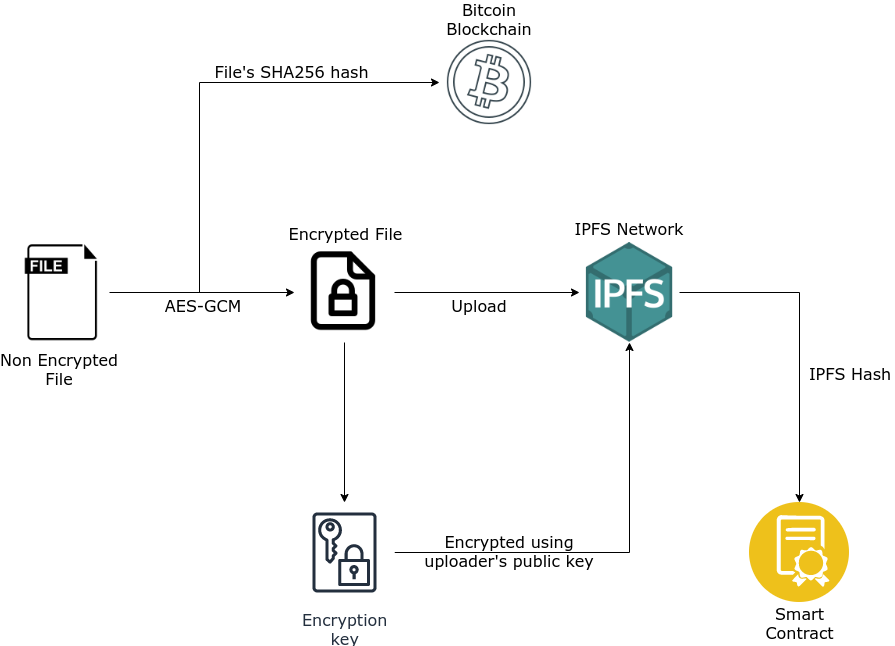
\includegraphics[width=\linewidth]{figures/ethereum-upload}
					\caption{\label{fig:ethereum-upload} File Upload using \textit{dshare-ethereum}}
				\end{figure}
				
				As soon as a user submits a file to be uploaded, it's SHA-256\footnote{\url{https://www.movable-type.co.uk/scripts/sha256.html}} hash is calculated and a timestamp is created by submitting the hash to the bitcoin blockchain using the OriginStamp API\footnote{\url{http://doc.originstamp.org/}}.
				
				Next, the file is encrypted using the SubtleCrypto\footnote{\url{https://developer.mozilla.org/en-US/docs/Web/API/SubtleCrypto}} interface with 'AES-GCM'\footnote{\url{https://en.wikipedia.org/wiki/Galois/Counter_Mode}} as the encryption algorithm. The encrypted data is then combined with the random salt to generate a \texttt{Uint8Array} buffer ready to be uploaded to the IPFS network.
				
				The key used to encrypt the file is converted to \texttt{JSON} and is encrypted using the uploader's Ethereum public key which is retrieved from the database. This encrypted key and the encrypted data is then uploaded to the IPFS network. Once the file is successfully uploaded, \texttt{createFile()} in the \texttt{FileFactory} contract is called which deploys a new \texttt{File} contract with all details regarding the file saved to the blockchain.
			
			\subsubsection{File Sharing}
				Sharing a file requires the recipient's Ethereum address and uploader's private key. Figure~\ref{fig:ethereum-share} visualizes the working of the application when a user shares a file with another user. Reference code is available at \url{https://github.com/hKedia/dShare/blob/master/components/FileSharing.js}
				
				\begin{figure}[h]
					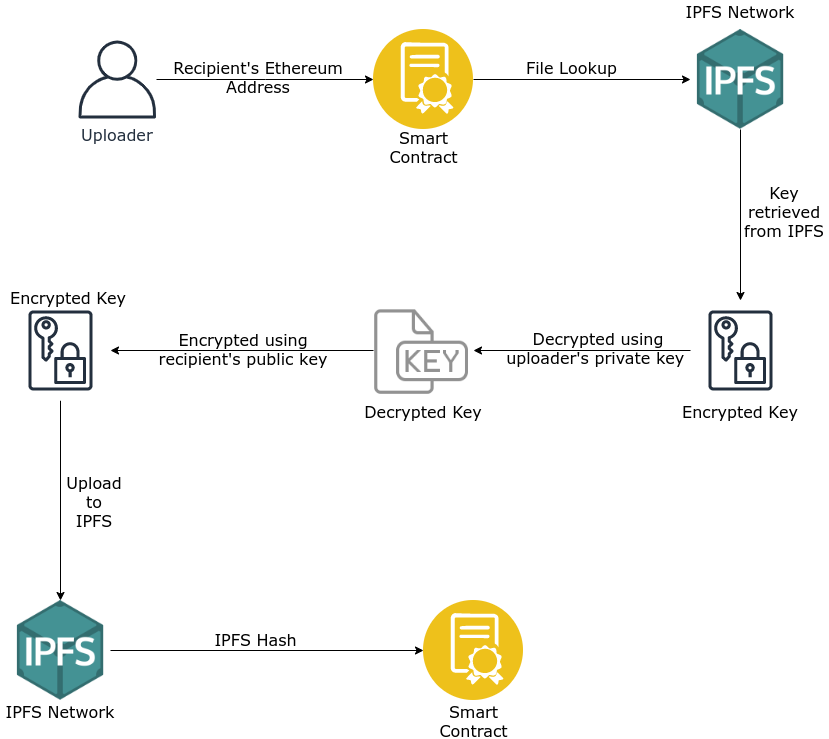
\includegraphics[width=\linewidth]{figures/ethereum-share}
					\caption{\label{fig:ethereum-share} File Sharing using \textit{dshare-ethereum}}
				\end{figure}
				
				Firstly, the file's IPFS location is retrieved from the \texttt{File} contract. From this location, the encrypted key is download and decrypted using uploader's private key. Once decrypted, the key is again encrypted using a recipient's public key. The new encrypted key is again uploaded to the IPFS network. Finally, the IPFS location of the key is saved into the \texttt{File} contract by calling \texttt{shareFile()}.
				
				To stop sharing a file, a function call can be made to the \texttt{File} contract with the recipient's address, which deletes the contract reference from the \texttt{recipientFiles} array.
			
			\subsubsection{File Download}
				Downloading a file requires the user's Ethereum private key. Depending on whether the file is uploaded or shared one, corresponding function from the \texttt{File} contract is called to retrieve the file's details. The key is then decrypted using user's private key and is converted to a valid JSON web key (jwk)\footnote{\url{https://tools.ietf.org/html/rfc7517}} format. The encrypted file data is then converted to a file buffer, and the original file content and the random salt used for encrypting the file is retrieved. Finally, the file is decrypted and saved to the user's local storage. Reference code for file download is available at \url{https://github.com/hKedia/dShare/blob/master/components/FileDownload.js}
			
			\subsubsection{File Archiving}
				Instead of deleting a \texttt{File} contract, the application provides a way to achieve files. This is also useful to keep track of archived files and restore them at a later date if required. When a file is archived, the \texttt{File} contract address is saved in an array which is later used for filtering the archived files from the UI. Restoring a file removes the \texttt{File} contract address from the archived files array. The reference code for file archiving is available at \url{https://github.com/hKedia/dShare/blob/master/components/FileDetail.js#L71}
				
			\subsubsection{Limitations}
			This application is built using experimental p2p technologies that is changing very rapidly. Below are some of the limitations:
			
			\begin{itemize}
				\item IPFS nodes treat the stored data as cache, meaning there is no guarantee the data will continue to be available. To overcome this, users should run their own IPFS nodes and \textit{pin}\footnote{\url{https://docs.ipfs.io/guides/concepts/pinning/}} the data that is important.
				\item MetaMask, the Ethereum wallet used in the application has no function that allows us retrieve the private key of the user within the application. Therefore, whenever a user wants to share or download a file, the private key must be manually provided for decryption.
			\end{itemize}
			
	\section{A File Sharing Application using Blockstack}
		This section describes the workings of the application \textit{dshare-blockstack}\cite{harsh_kedia_2019_3359854} built using Blockstack\footnote{\url{https://blockstack.org/}}, a decentralized computing network and app ecosystem. The latest version of the application is deployed at \url{https://dshare-blockstack.herokuapp.com/}.
		
		\subsection{Use Case}
		\textit{dshare-blockstack} focus on easy sharing of files between two users. The encryption and decryption is handled by keys generated on user's machine. It leverages the existing cloud infrastructure for storage thereby providing a rich user experience.
		
		\subsection{Technologies Used}
			\subsubsection{Blockstack}
			Blockstack\cite{ali2016blockstack} is a platform for building highly scalable decentralized applications where users own their data. It implements a DPKI system (see Section~\ref{sec:blockstack-auth}) anchored on the Bitcoin blockchain. It also implements a storage system, Gaia (see Section~\ref{sec:blockstack-gaia}) which leverages the existing cloud infrastructure providing users with private data lockers.
			
			\subsubsection{Radiks}
			"Radiks\footnote{\url{https://github.com/blockstack-radiks/radiks-server}} is a framework for building complex and collaborative decentralized applications, using Blockstack infrastructure under the hood"\footnote{\url{https://blog.blockstack.org/introducing-radiks/}}. It serves as a indexing server for data that is stored in Gaia. \textit{dshare-blockstack} uses the front-end component library, \textit{radiks.js}\footnote{\url{https://github.com/blockstack-radiks/radiks}} for interacting with Radiks.
		
		\subsection{Application Architecture}
			Figure~\ref{fig:dshare-blockstack} visualizes the application architecture. User authentication is handled by the Blockstack browser\footnote{\url{https://browser.blockstack.org/}}. Files are uploaded to the user's Gaia Hub, a private data locker in the cloud. Before uploading, files are encrypted using a symmetric key employing AES-GCM as the encryption mechanism. Sharing logic is implemented using Radiks which provides an API for creating models to represent uploaded files.
		
			\begin{figure}[h]
				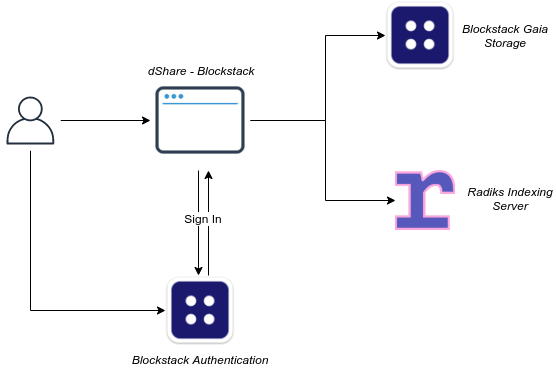
\includegraphics[width=\linewidth]{figures/dshare-blockstack}
				\caption{\label{fig:dshare-blockstack} \textit{dShare-blockstack} Architecture}
			\end{figure}
		
		\subsection{Working}
		
			\subsubsection{Authentication}
			When a user sings into the application, she is redirected to the Blockstack browser. Here she can create a new Blockstack ID or select on of her existing IDs. See Section~\ref{sec:blockstack-auth} for the authentication flow. Once authenticated, user is redirected back to the application and logged in. The public key of the user is saved under \textit{/keys} inside her Gaia hub which is later used for encrypting a file's encryption key.
			
			\subsubsection{File Upload}
			Figure~\ref{fig:blockstack-upload} visualizes the working of the application when a user uploads a file.
			
			\begin{figure}[h]
				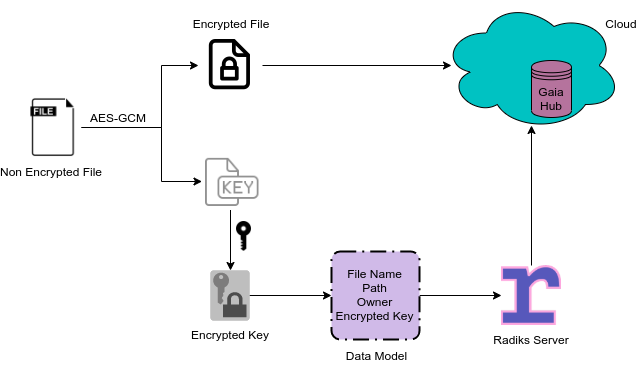
\includegraphics[width=\linewidth]{figures/blockstack-upload}
				\caption{\label{fig:blockstack-upload} File Upload using \textit{dShare-blockstack}}
			\end{figure}
			
			\subsubsection{File Sharing}
			
			\subsubsection{File Download}
			
			\subsubsection{File Deletion}
			
			\subsubsection{Limitations}